\documentclass{article}
\usepackage[english,UKenglish]{babel}
\usepackage{hyperref}
\usepackage{url}
\usepackage{fullpage}
\usepackage{graphicx}
\usepackage{tabularx}
\usepackage{amssymb}
\usepackage{stackrel}
\usepackage{array}
\usepackage{amsmath}
\usepackage{verbatim}
\usepackage{multirow}
\usepackage{rotating}
\usepackage{fancybox}
\usepackage{pdflscape}
\usepackage{amsthm}
\usepackage{blkarray}
\usepackage{algorithmic}
\usepackage{algorithm}
\begin{document}
\begin{figure}[tbh]
\begin{minipage}[c]{0.49\textwidth}\centering
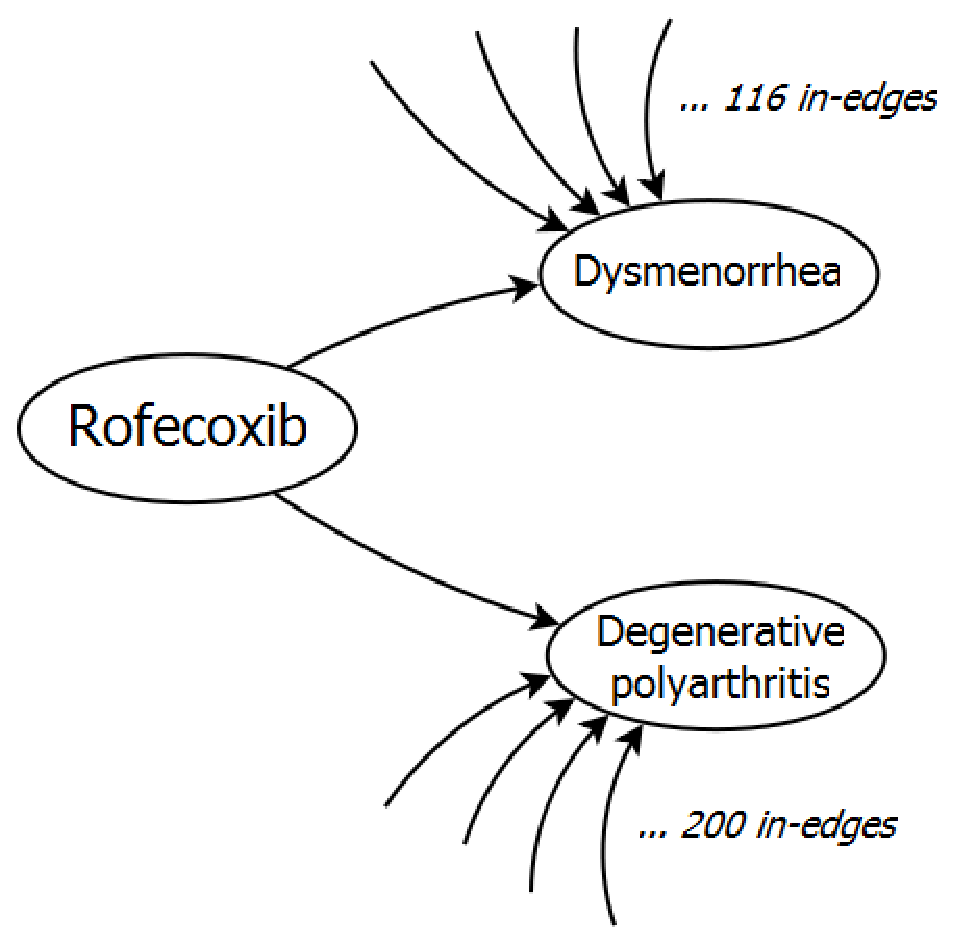
\includegraphics[width=.7\textwidth]{fig/may_treat.eps}
\end{minipage}
\begin{minipage}[c]{0.49\textwidth}\centering
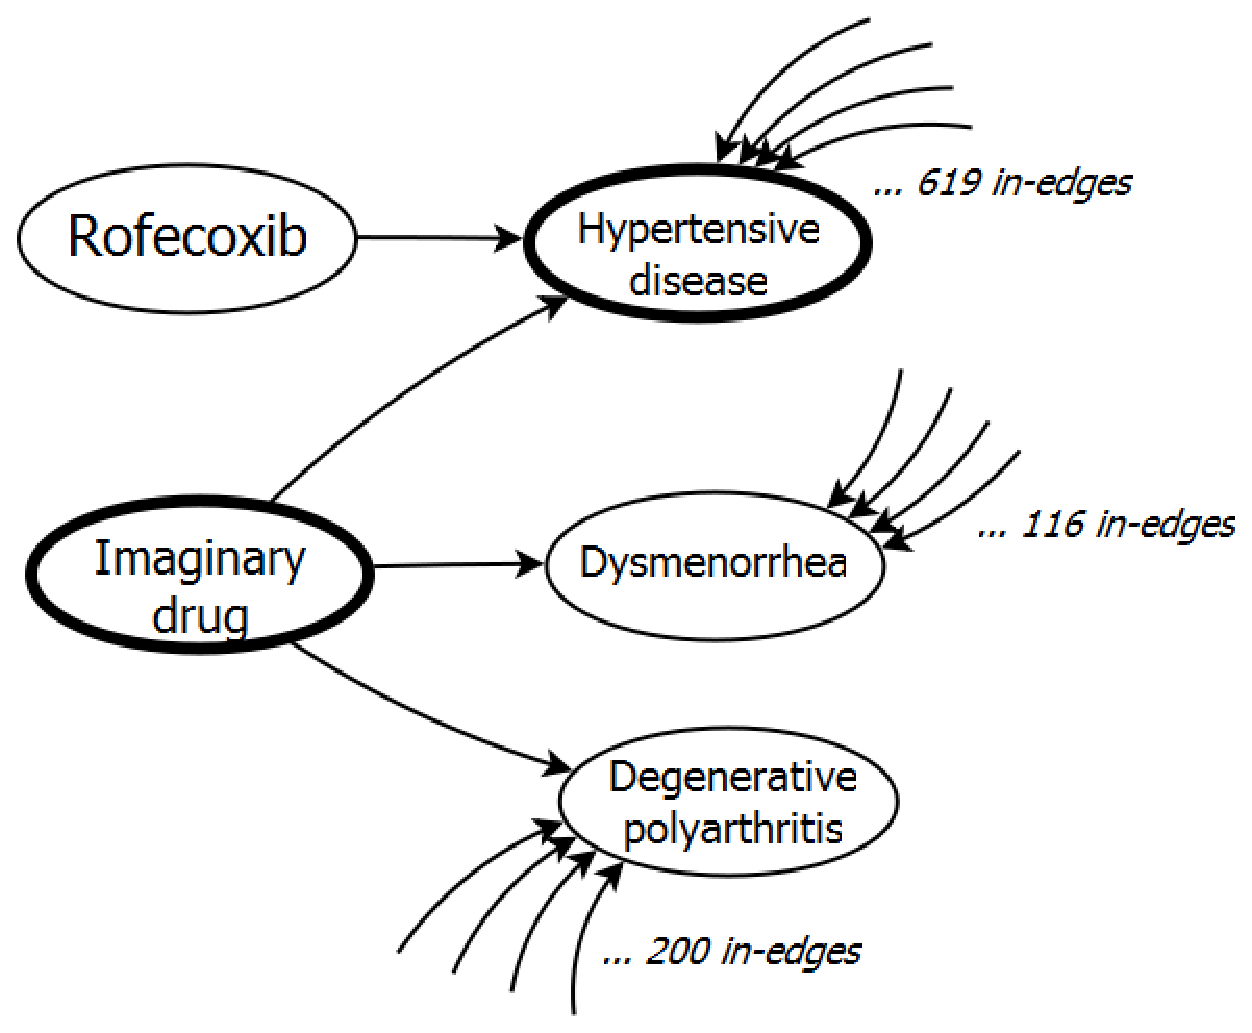
\includegraphics[width=.9\textwidth]{fig/may_treat_augmented.eps}
\end{minipage}
\caption[The may\_treat subgraph]{\label{fig:may_treat} The left-hand side of the figure shows the may\_treat subgraph of ground truth relationships between the drug Rofecoxib and two diseases. The right-hand side shows the ``salted" may\_treat subgraph with deliberately distorted information.}
\end{figure}

\begin{table*}[tbh]\scriptsize
\begin{center}
\begin{tabular}{ c || c  c || c  c }
\hline
        &   \multicolumn{2}{c||}{w/ ``salted" may\_treat only}    &   \multicolumn{2}{c}{w/ data and ``salted" may\_treat}\\
\hline
\hline
       	&   p(\%)   &   rank    &  p(\%)    &    rank    \\
\hline
$\langle Rofecoxib, degenerative~polyarthritis\rangle$       &   3.60e-3   &   555     &   8.14e-3    &   263    \\
$\langle Rofecoxib, dysmenorrhea\rangle$    &   1.54e-2   &   246     &   1.26e-3    &   1703   \\
\hline
\end{tabular}
\end{center}
\caption[Rankings of associations on the ``salted" may\_treat graph]{\label{tbl:salted_may_treat}Rankings of associations between Rofecoxib and two diseases on the ``salted" may\_treat graph (Figure~\ref{fig:may_treat} right) derived with and without data.}
\end{table*}

On the other hand, we are also interested in learning whether the data graph can help discover patterns in the ontology graph. Figure~\ref{fig:may_treat} (left) shows a subgraph of the NDFRT ``may\_treat" relationship. Rofecoxib is asserted to treat two diseases, namely, dysmenorrhea and degenerative polyarthritis. And there are altogether 116 and 200 drugs that are known to treat dysmenorrhea and degenerative polyarthritis respectively (hence the in-degrees of the nodes). Applying our method on this graph with the query term ``Rofecoxib" yields a similarity-ranked list having degenerative polyarthritis and dysmenorrhea as the top two items. Since this result is the exact ground truth, there is no improvement to be made with the incorporation of the data graph. Therefore, we ``salt" the ground truth graph with some deliberately distorted information, as is shown in Figure~\ref{fig:may_treat} (right), so that the may\_treat graph alone produces only inferior result. More specifically, we specify that Rofecoxib should treat hypertensive disease, the very diseases that is asserted to be treated by the most drugs (a total of 619). Then we add an imaginary drug to treat degenerative polyarthritis, dysmenorrhea, and hypertensive disease. In this way, the original direct connections between Rofecoxb and degenerative polyarthritis and dysmenorrhea become erroneously indirect and are obfuscated by some the noise of high degree nodes along the path. With this scenario, we hope to learn if the incorporation of data graph can correct the misinformation in ontologies.

Table~\ref{tbl:salted_may_treat} shows the result of ranks of the associations between Rofecoxib and degenerative polyarthritis and dysmenorrhea. The ranks of the associations drastically drop to the 555th and 246th respectively on the ``salted" graph from the top two on the original ground truth graph. This is mainly due to the large node, hypertensive disease, in the middle of the connections. However, with the combined data and may\_treat graph, we notice that the rank of Rofecoxib and degenerative polyarthritis increases to 263rd, while the rank of Rofecoxib and  dysmenorrhea decreases to 1703rd. This shows that the data graph endorses more strongly the association between Rofecoxib and degenerative polyarthritis. Indeed, although Rofecoxib are known to treat both degenerative polyarthritis and dysmenorrhea, the former is a much more popular usage. A search on the National Library of Medicine's PubMed database\footnotemark[1] for ``Rofecoxib and polyarthritis" returns 518 results, while ``Rofecoxib and dysmenorrhea" only returns 29. This result shows that the data graph can help correct misinformation in ontologies to some extent, and in a sense, it also gives a clue of how prior beliefs fit with reality.

\footnotetext[1]{\url{http://www.ncbi.nlm.nih.gov/}}
\end{document}